\documentclass[11pt,a4paper]{article}
\usepackage[T1]{fontenc}
\usepackage[utf8]{inputenc}
\usepackage{lmodern}
\usepackage[margin=2.3cm]{geometry}
\usepackage{amsmath,amssymb,bm}
\usepackage{graphicx,booktabs,array,tabularx}
\usepackage{tikz}
\usetikzlibrary{arrows.meta,calc,patterns}
\usepackage[font=small,labelfont=bf]{caption}
\usepackage{xcolor}
\definecolor{accent}{HTML}{1D58B8}
\definecolor{hot}{HTML}{D9561A}
\usepackage[colorlinks=true,linkcolor=accent,citecolor=accent,urlcolor=accent]{hyperref}
\usepackage{enumitem}
\setlist{nosep,leftmargin=*}

\newcommand{\MPam}{\,\mathrm{MPa}\sqrt{\mathrm{m}}}
\newcommand{\dd}{\mathrm{d}}
\newcommand{\Kt}{K_t}
\renewcommand{\Re}{\operatorname{Re}}
\renewcommand{\Im}{\operatorname{Im}}

\title{Stress Intensity at the Crack Tip\\[4pt]\large Lecture notes accompanying the interactive pages}
\author{Dr R\'egis Kubler\\ \normalsize Arts et M\'etiers Institute of Technology\\[4pt] \small Written with the assistance of Claude Opus 5.5 (Anthropic)}
\date{October 2026}

\begin{document}
\maketitle

\begin{abstract}
These notes collect every equation and graph shown in the two interactive pages
\emph{Stress intensity at the crack tip} and \emph{Angular functions $f_{ij}(\theta)$}.
They follow the same order: stress concentration at an elliptical hole (Section~\ref{sec:kt}),
the crack-tip singularity (Section~\ref{sec:sing}), the near-tip field and the definition of $K$
(Section~\ref{sec:williams}), handbook solutions (Section~\ref{sec:handbook}), extraction of $K$
from numerical results (Section~\ref{sec:fe}), the fracture criterion (Section~\ref{sec:frac}),
and the angular functions for all three modes with mixed-mode loading and the $T$-stress
(Section~\ref{sec:angular}). All figures were computed from the closed-form solutions given in the
text by the script \texttt{make\_figures.py} supplied with this document.
\end{abstract}

\tableofcontents
\bigskip

%=====================================================================
\section{Coordinates and notation}\label{sec:coords}
%=====================================================================
Throughout, the crack lies in the plane $y=0$ and its front is parallel to $z$.
Two coordinate systems are used (Figure~\ref{fig:coords}).

\begin{itemize}
  \item \textbf{Global coordinates} $(x,y)$ for a through crack of length $2a$: the origin is the
  \emph{centre} of the crack, so the crack occupies $-a\le x\le a$ and the tips are at $x=\pm a$.
  \item \textbf{Crack-tip polar coordinates} $(r,\theta)$: the origin is the \emph{tip}; $r$ is the
  distance from the tip and $\theta$ is measured anticlockwise from the crack line ahead of the tip.
  Hence $\theta=0$ is straight ahead and $\theta=\pm\pi$ are the upper and lower crack faces. For the
  right-hand tip of a centre crack, $r=x-a$ on the line $y=0$.
\end{itemize}

\begin{figure}[!htbp]
\centering
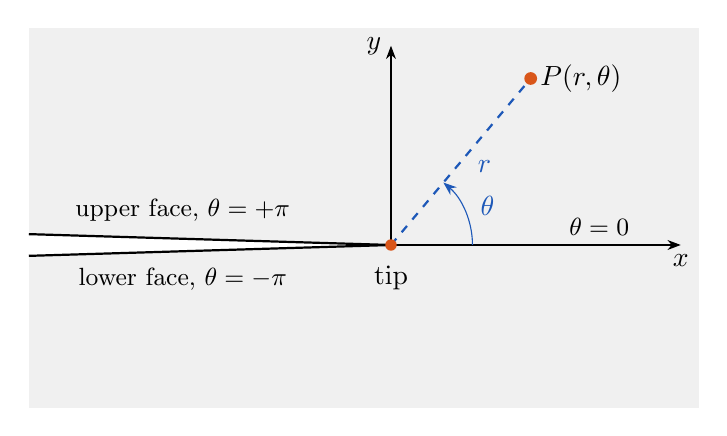
\begin{tikzpicture}[scale=1.15,>=Stealth]
  \fill[black!6] (-4,-1.8) rectangle (3.4,2.4);
  \fill[white] (-4,0.12) -- (0,0) -- (-4,-0.12) -- cycle;
  \draw[thick] (-4,0.12) -- (0,0) -- (-4,-0.12);
  \draw[->] (0,0) -- (3.2,0) node[below] {$x$};
  \draw[->] (0,0) -- (0,2.2) node[left] {$y$};
  \draw[accent,thick,dashed] (0,0) -- (50:2.4) coordinate (P);
  \fill[hot] (P) circle (2pt) node[right,black] {$P(r,\theta)$};
  \node[accent] at (40:1.35) {$r$};
  \draw[accent,->] (0.9,0) arc (0:50:0.9);
  \node[accent] at (22:1.15) {$\theta$};
  \fill[hot] (0,0) circle (1.8pt);
  \node[below] at (0,-0.12) {tip};
  \node[above,font=\small] at (-2.3,0.15) {upper face, $\theta=+\pi$};
  \node[below,font=\small] at (-2.3,-0.15) {lower face, $\theta=-\pi$};
  \node[font=\small,above] at (2.3,0) {$\theta=0$};
\end{tikzpicture}
\caption{Crack-tip polar coordinates. The angular functions $f_{ij}(\theta)$ are always written in this
frame, attached to the crack itself, whatever the orientation of the crack relative to the load.}
\label{fig:coords}
\end{figure}

Elastic constants: Young's modulus $E$, Poisson's ratio $\nu$, shear modulus $\mu=E/2(1+\nu)$, and
\begin{equation}
  E' = \begin{cases} E & \text{plane stress}\\ E/(1-\nu^2) & \text{plane strain}\end{cases},\qquad
  \kappa = \begin{cases} (3-\nu)/(1+\nu) & \text{plane stress}\\ 3-4\nu & \text{plane strain.}\end{cases}
\end{equation}
Units: stresses in MPa, lengths in metres inside $\sqrt{\pi a}$, so that $K$ is in $\MPam$.

%=====================================================================
\section{Stress concentration at an elliptical hole}\label{sec:kt}
%=====================================================================
\subsection{Geometry and the Inglis result}
An infinite plate is loaded by a remote uniaxial stress $\sigma_\infty$ in the $y$-direction and contains
an elliptical hole with semi-axis $a$ along $x$ (across the load) and $b$ along $y$. The radius of
curvature at the end of the major axis is
\begin{equation}
  \rho = \frac{b^2}{a}.
\end{equation}
Inglis (1913) showed that the maximum stress, at $(x,y)=(\pm a,0)$, is
\begin{equation}\label{eq:inglis}
  \sigma_{\max} = \sigma_\infty\left(1+\frac{2a}{b}\right)
  = \sigma_\infty\left(1+2\sqrt{\frac{a}{\rho}}\right),
  \qquad
  \Kt = \frac{\sigma_{\max}}{\sigma_\infty} = 1 + 2\sqrt{\frac{a}{\rho}} .
\end{equation}
A circular hole ($b=a$) gives the familiar $\Kt=3$; at the top of the hole $(0,\pm b)$ the hoop
stress is $-\sigma_\infty$.

\subsection{Full field: Kolosov--Muskhelishvili solution}
The field plotted in Figure~\ref{fig:ellipse} is computed from complex potentials. Two complex
variables are used:
\begin{itemize}
  \item $z = x+iy = re^{i\theta}$ is the \emph{physical} position in the plate, with the origin at the
  centre of the hole ($\bar z = x-iy$ is its conjugate);
  \item $\zeta = \rho_\zeta e^{i\eta}$ (zeta) is an auxiliary coordinate in a \emph{mapped} plane, chosen so that
  the hole boundary becomes the unit circle $|\zeta|=1$ and the plate becomes $|\zeta|\ge1$.
\end{itemize}
Working in $\zeta$ turns the elliptical boundary into a circle, where the boundary condition is easy
to impose. On the hole, $\zeta=e^{i\eta}$ and the mapping below gives $x=a\cos\eta$, $y=b\sin\eta$:
the angle $\eta$ is the eccentric angle of the ellipse, and $|\zeta|\to\infty$ corresponds to
$|z|\to\infty$. The mapping is
\begin{equation}
  z = \omega(\zeta) = R\left(\zeta + \frac{m}{\zeta}\right),\qquad
  R=\frac{a+b}{2},\quad m = \frac{a-b}{a+b},
\end{equation}
with inverse $\zeta = \bigl(z+\sqrt{z^2-4R^2m}\bigr)/2R$ (root with $|\zeta|\ge 1$).
For uniaxial tension $\sigma_\infty$ along $y$ the potentials are
\begin{align}
  \varphi(\zeta) &= \frac{\sigma_\infty R}{4}\left(\zeta - \frac{2+m}{\zeta}\right),\\
  \psi(\zeta) &= -\frac{\sigma_\infty R}{2}\left[-\zeta - \frac{1}{m\zeta}
      + \frac{(1+m)(1+m^2)}{m}\,\frac{\zeta}{\zeta^2-m}\right],
\end{align}
and the stresses follow from the Kolosov--Muskhelishvili relations
\begin{align}
  \sigma_{xx}+\sigma_{yy} &= 4\,\Re\,\Phi(z), \\
  \sigma_{yy}-\sigma_{xx}+2i\tau_{xy} &= 2\left[\bar z\,\Phi'(z)+\Psi(z)\right],
\end{align}
with $\Phi = \varphi'(\zeta)/\omega'(\zeta)$, $\Phi'(z) = \Phi_{,\zeta}/\omega'(\zeta)$ and
$\Psi = \psi'(\zeta)/\omega'(\zeta)$. Primes on $\varphi,\psi,\omega$ denote derivatives with
respect to $\zeta$; $\Phi$ and $\Psi$ are the derivatives with respect to $z$, obtained by the chain rule
$\dd/\dd z = (1/\omega')\,\dd/\dd\zeta$. Explicitly,
\begin{align}
  \omega'(\zeta) &= R\left(1-\frac{m}{\zeta^2}\right), &
  \omega''(\zeta) &= \frac{2Rm}{\zeta^3},\\
  \varphi'(\zeta) &= \frac{\sigma_\infty R}{4}\left(1+\frac{2+m}{\zeta^2}\right), &
  \varphi''(\zeta) &= -\frac{\sigma_\infty R}{2}\,\frac{2+m}{\zeta^3},\\
  \psi'(\zeta) &= -\frac{\sigma_\infty R}{2}\left[-1+\frac{1}{m\zeta^2}-\frac{(1+m)(1+m^2)}{m}\,\frac{\zeta^2+m}{(\zeta^2-m)^2}\right],
\end{align}
and
\begin{equation}
  \Phi'(z) = \frac{1}{\omega'}\,\frac{\dd\Phi}{\dd\zeta}
  = \frac{\varphi''\omega'-\varphi'\omega''}{\omega'^{\,3}} .
\end{equation} These potentials were checked numerically: they give
$\sigma_{yy}(a,0)=\sigma_\infty(1+2a/b)$, $\sigma_{xx}(0,b)=-\sigma_\infty$, zero traction on the
hole boundary, and $\sigma_{yy}\to\sigma_\infty$ far away.

\begin{figure}[!htbp]
\centering
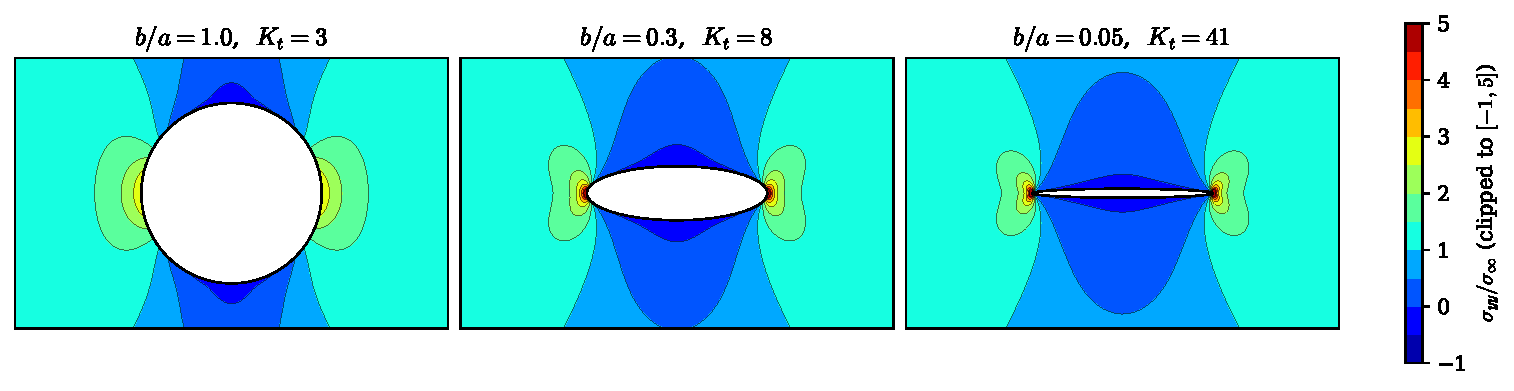
\includegraphics[width=\textwidth]{figures/ellipse_fields.pdf}
\caption{Opening stress $\sigma_{yy}/\sigma_\infty$ around an elliptical hole as it flattens from a
circle into a crack. The peak at the end of the hole rises as $1+2a/b$.}
\label{fig:ellipse}
\end{figure}

\subsection{From $\Kt$ to $K$: the sharp-crack limit}
$\Kt$ depends only on the \emph{shape} of the hole: scaling $a$ and $b$ together leaves
$\sigma_{\max}$ unchanged. When $b\to 0$ the ellipse becomes a crack of length $2a$, $\rho\to 0$ and
$\Kt\to\infty$, so the stress concentration factor stops being useful. Multiplying
\eqref{eq:inglis} by $\tfrac{\sqrt{\pi}}{2}\sqrt{\rho}$,
\begin{equation}
  \frac{\sqrt{\pi}}{2}\,\sigma_{\max}\sqrt{\rho}
  = \sigma_\infty\left(\sqrt{\pi a} + \frac{\sqrt{\pi\rho}}{2}\right),
\end{equation}
which stays finite and, in the limit of a sharp crack, gives the stress intensity factor (Irwin):
\begin{equation}\label{eq:irwinlimit}
  \boxed{\,K_I = \lim_{\rho\to 0}\ \frac{\sqrt{\pi}}{2}\,\sigma_{\max}\sqrt{\rho} = \sigma_\infty\sqrt{\pi a}\,}
\end{equation}
In normalised form the ratio plotted in Figure~\ref{fig:ktlimit} is
\begin{equation}
  \frac{(\sqrt\pi/2)\,\sigma_{\max}\sqrt\rho}{\sigma_\infty\sqrt{\pi a}}
  = 1 + \frac12\sqrt{\frac{\rho}{a}} = 1 + \frac{b}{2a}\ \xrightarrow{\ \rho\to0\ }\ 1 .
\end{equation}

\begin{figure}[!htbp]
\centering
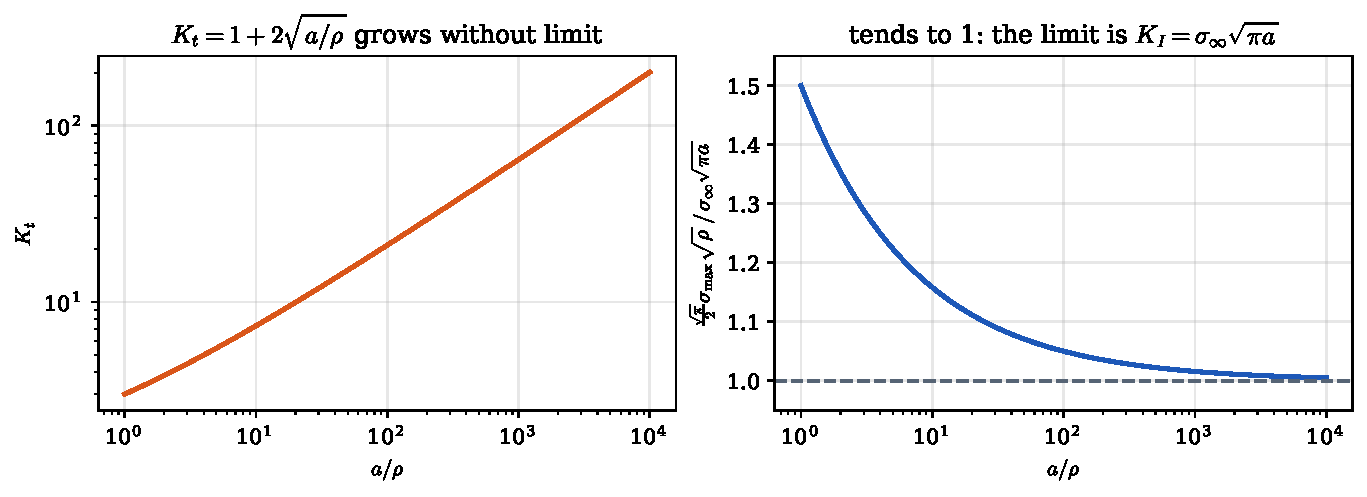
\includegraphics[width=.92\textwidth]{figures/kt_limit.pdf}
\caption{Left: $\Kt$ grows without limit as the hole sharpens. Right: the product
$(\sqrt\pi/2)\sigma_{\max}\sqrt\rho$ tends to $\sigma_\infty\sqrt{\pi a}$, which is $K_I$ for the crack.}
\label{fig:ktlimit}
\end{figure}

\begin{table}[!htbp]
\centering
\caption{Stress concentration factor and stress intensity factor compared.}
\begin{tabular}{@{}lll@{}}
\toprule
 & $\Kt$, stress concentration & $K$, stress intensity\\
\midrule
Applies to & blunt notches and holes, $\rho$ finite & sharp cracks, $\rho\to0$\\
Units & none & $\MPam$\\
Depends on & shape only & shape, size and load\\
Peak stress & finite, $\sigma_{\max}=\Kt\sigma$ & infinite, $\sigma\propto K/\sqrt{2\pi r}$\\
Compared with & yield or fatigue strength & fracture toughness $K_{IC}$\\
\bottomrule
\end{tabular}
\end{table}

%=====================================================================
\section{The crack-tip singularity}\label{sec:sing}
%=====================================================================
\subsection{Westergaard solution for a centre crack}
For a crack $-a\le x\le a$ in an infinite plate under remote equibiaxial stress $\sigma_\infty$,
Westergaard's stress function is
\begin{equation}
  Z(z) = \frac{\sigma_\infty z}{\sqrt{z^2-a^2}},\qquad
  Z'(z) = -\frac{\sigma_\infty a^2}{(z^2-a^2)^{3/2}},
\end{equation}
with the branch cut on the crack, and
\begin{equation}
  \sigma_{xx} = \Re Z - y\,\Im Z',\qquad
  \sigma_{yy} = \Re Z + y\,\Im Z',\qquad
  \tau_{xy} = -y\,\Re Z'.
\end{equation}
For uniaxial loading normal to the crack, subtract $\sigma_\infty$ from $\sigma_{xx}$; $\sigma_{yy}$
and $\tau_{xy}$ are unchanged. On the crack line ($y=0$, $|x|>a$):
\begin{equation}\label{eq:crackline}
  \sigma_{yy}(x,0) = \frac{\sigma_\infty\,x}{\sqrt{x^2-a^2}},
\end{equation}
where $x$ is measured from the centre of the crack. This stress tends to infinity as $x\to a$.

\subsection{Recovering the $1/\sqrt r$ term}
Put $x=a+r$ in \eqref{eq:crackline}:
\begin{equation}
  \sigma_{yy}(r,0) = \frac{\sigma_\infty(a+r)}{\sqrt{r(2a+r)}}
  = \frac{\sigma_\infty\sqrt{\pi a}}{\sqrt{2\pi r}}\;\frac{1+r/a}{\sqrt{1+r/2a}}
  \;\xrightarrow{\ r\ll a\ }\; \frac{\sigma_\infty\sqrt{\pi a}}{\sqrt{2\pi r}} = \frac{K_I}{\sqrt{2\pi r}}.
\end{equation}
Halving the distance from the tip raises the stress by $\sqrt2$, not by $2$. The stress at the tip is
therefore not a useful number for a sharp crack; the \emph{amplitude} of the singularity, $K_I$, is.

\begin{figure}[!htbp]
\centering
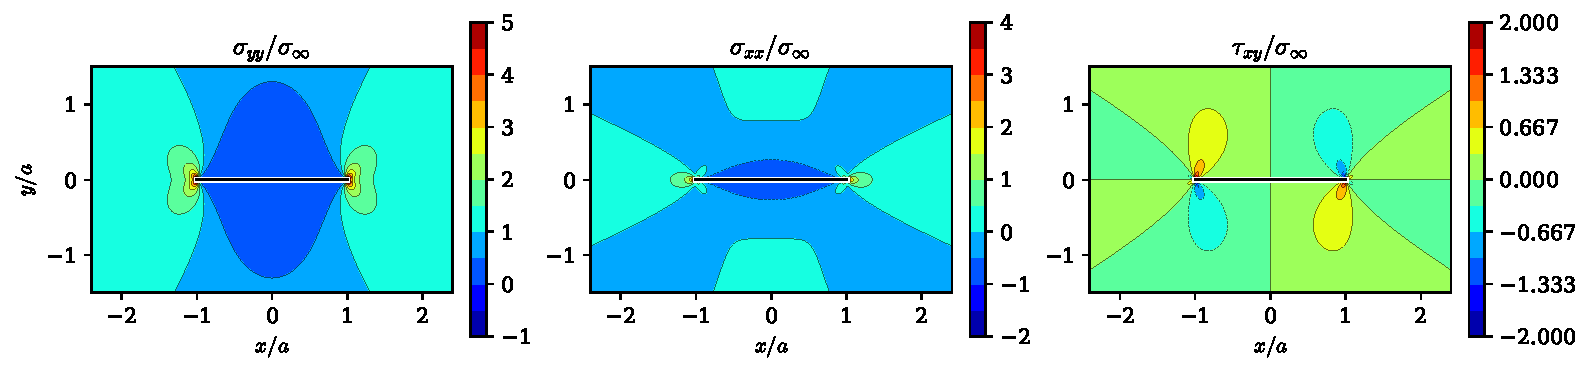
\includegraphics[width=\textwidth]{figures/westergaard_fields.pdf}\\[4pt]
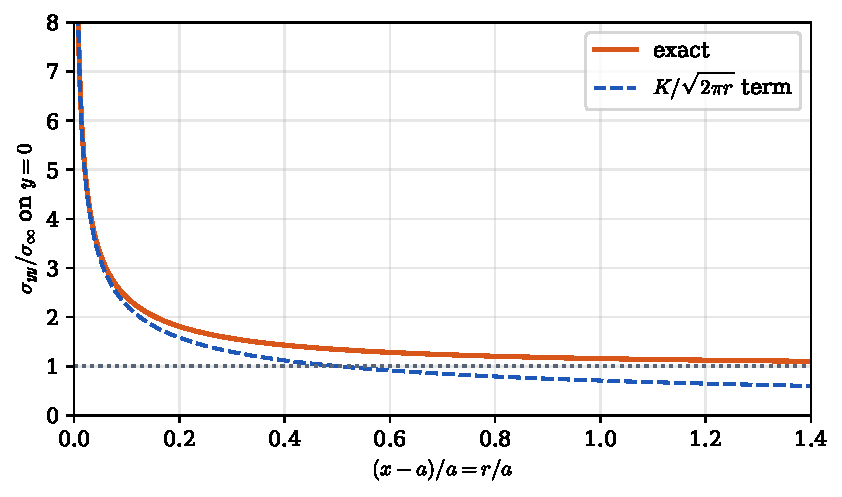
\includegraphics[width=.6\textwidth]{figures/westergaard.pdf}
\caption{Top: Westergaard stress components around a centre crack under uniaxial tension (rainbow
scale, blue = minimum, red = maximum, clipped near the tips). Bottom: $\sigma_{yy}$ along the crack
line ahead of the right tip, compared with its singular term $K_I/\sqrt{2\pi r}$.}
\end{figure}

%=====================================================================
\section{The near-tip field and the definition of $K$}\label{sec:williams}
%=====================================================================
Williams (1957) showed that, close to the tip of any crack in a linear elastic body, the stresses take
the form
\begin{equation}\label{eq:williams}
  \sigma_{ij}(r,\theta) = \frac{K}{\sqrt{2\pi r}}\,f_{ij}(\theta) + \text{(terms that are finite as } r\to0).
\end{equation}
For mode I,
\begin{align}
  f^{I}_{xx}(\theta) &= \cos\tfrac{\theta}{2}\left[1-\sin\tfrac{\theta}{2}\sin\tfrac{3\theta}{2}\right],\\
  f^{I}_{yy}(\theta) &= \cos\tfrac{\theta}{2}\left[1+\sin\tfrac{\theta}{2}\sin\tfrac{3\theta}{2}\right],\\
  f^{I}_{xy}(\theta) &= \cos\tfrac{\theta}{2}\,\sin\tfrac{\theta}{2}\,\cos\tfrac{3\theta}{2}.
\end{align}
Geometry, crack length and load all enter through the single scalar $K_I$. Since $f^I_{yy}(0)=1$,
\begin{equation}\label{eq:Kdef}
  K_I = \lim_{r\to 0}\ \sigma_{yy}(r,0)\sqrt{2\pi r},
  \qquad\text{and in general}\qquad
  K_I = \frac{\sigma_{ij}(r,\theta)\sqrt{2\pi r}}{f_{ij}(\theta)}\ \text{ for } r\to0,\ f_{ij}\ne0.
\end{equation}
The ratio is undefined where $f_{ij}=0$, for example $\tau_{xy}$ on $\theta=0$.

\begin{figure}[!htbp]
\centering
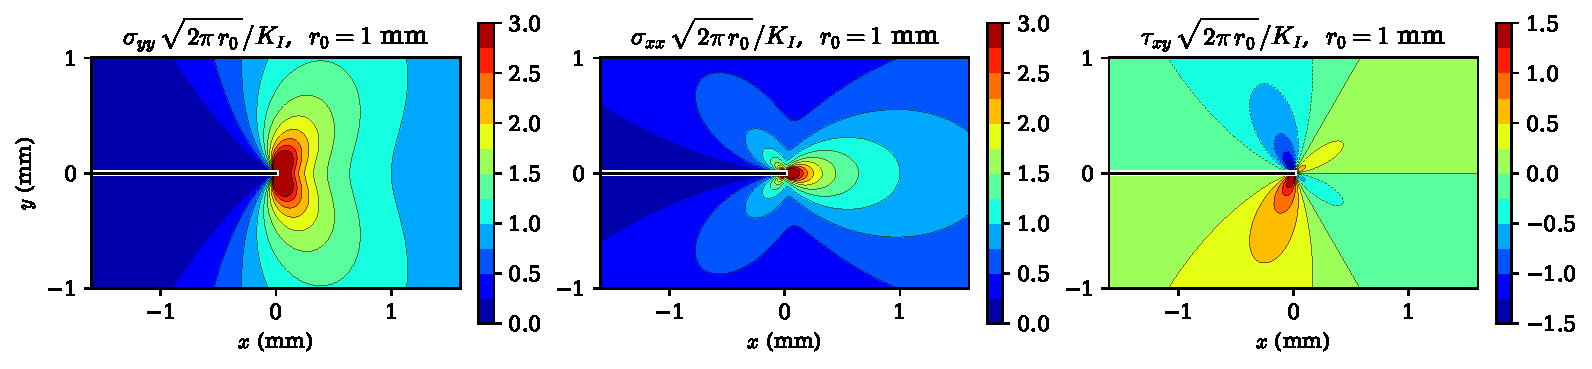
\includegraphics[width=\textwidth]{figures/williams_fields.pdf}
\caption{Mode I near-tip stress components $\sigma_{ij}=K_I f_{ij}(\theta)/\sqrt{2\pi r}$, normalised by
$K_I/\sqrt{2\pi r_0}$ with $r_0=1$\,mm; the crack lies along the negative $x$-axis. Rainbow scale,
blue = minimum, red = maximum.}
\end{figure}

\begin{figure}[!htbp]
\centering
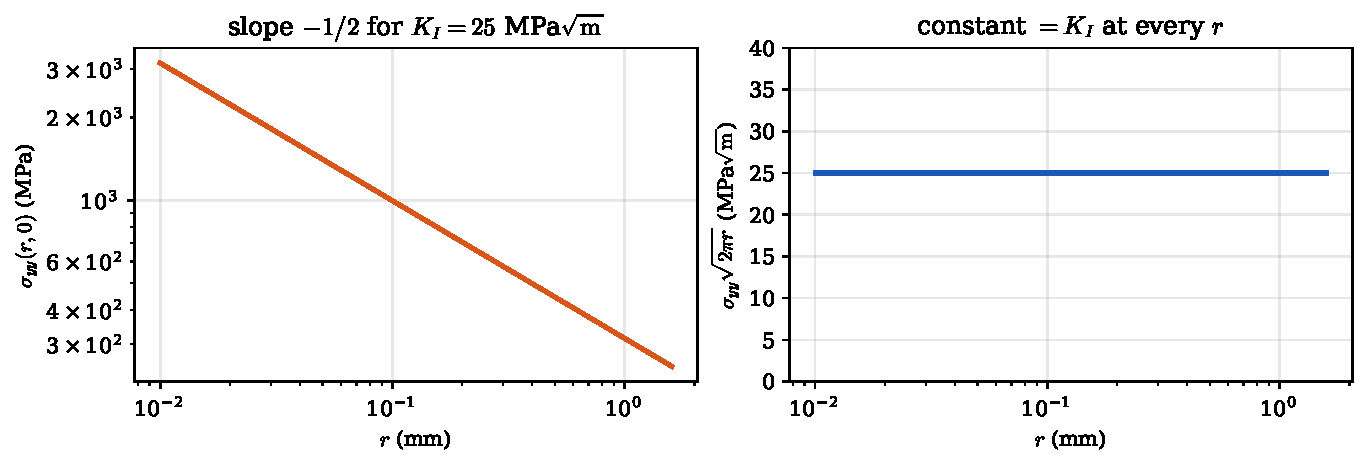
\includegraphics[width=.9\textwidth]{figures/singularity_slope.pdf}
\caption{Along $\theta=0$ the stress follows a slope of $-1/2$ on log--log axes, while
$\sigma_{yy}\sqrt{2\pi r}$ stays equal to $K_I$ at every distance. Example: $K_I=25\MPam$, $r$ in mm.}
\end{figure}

%=====================================================================
\section{Calculating $K$ from a handbook solution}\label{sec:handbook}
%=====================================================================
\subsection{The general form}
For standard geometries the elastic problem has been solved and tabulated as a dimensionless
geometry factor $Y$ (also written $F$ or $\beta$):
\begin{equation}
  K_I = Y\!\left(\frac aW\right)\sigma\sqrt{\pi a}.
\end{equation}
Procedure:
\begin{enumerate}
  \item identify the geometry and loading, and measure $a$ as the handbook defines it
  (half-length for a centre crack, full depth for an edge crack);
  \item read $Y$ at the current $a/W$ and check the range of validity;
  \item convert $a$ to metres;
  \item multiply out $K_I = Y\sigma\sqrt{\pi a}$.
\end{enumerate}

\subsection{Geometry factors used in the pages}
\begin{table}[!htbp]
\centering
\caption{Geometry factors for remote tension $\sigma$.}
\renewcommand{\arraystretch}{1.35}
\begin{tabular}{@{}p{4.6cm}p{6.4cm}p{3cm}@{}}
\toprule
Geometry & $Y$ & Validity\\
\midrule
Through crack $2a$, infinite plate (Griffith) & $1$ & exact\\
Edge crack $a$, semi-infinite plate & $1.122$ & exact\\
Centre crack $2a$, width $W$ (Feddersen) & $\sqrt{\sec(\pi a/W)}$ & $2a/W\le0.7$, $\pm0.3\%$\\
Single edge crack $a$, width $W$ (Tada) & $1.12-0.231\,\tfrac aW+10.55\left(\tfrac aW\right)^2$\newline$\quad-\,21.72\left(\tfrac aW\right)^3+30.39\left(\tfrac aW\right)^4$ & $a/W\le0.6$, $\pm0.5\%$\\
\bottomrule
\end{tabular}
\end{table}

\begin{figure}[!htbp]
\centering
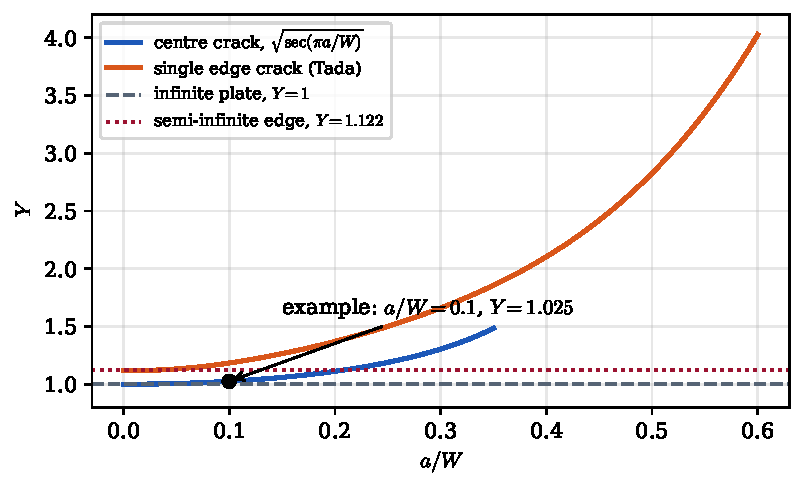
\includegraphics[width=.68\textwidth]{figures/geometry_factors.pdf}
\caption{Geometry factors against $a/W$.}
\end{figure}

\subsection{Worked example}
Centre crack, $a=20$\,mm, $W=200$\,mm, $\sigma=150$\,MPa:
\begin{align*}
  a/W &= 20/200 = 0.100,\\
  Y &= \sqrt{\sec(0.1\pi)} = 1.025,\\
  K_I &= 1.025\times150\,\mathrm{MPa}\times\sqrt{\pi\times0.0200\,\mathrm{m}} = 38.6\MPam.
\end{align*}

%=====================================================================
\section{Calculating $K$ from a numerical model}\label{sec:fe}
%=====================================================================
\subsection{Apparent $K$}
When no handbook solution exists, the part is modelled (for example by finite elements) and $K$ is
extracted from the near-tip results. Each node gives an \emph{apparent} $K$ by inverting the singular
term at its own distance $r$.

\paragraph{Stress method} (nodes ahead of the tip, $\theta=0$):
\begin{equation}
  K_{\rm app}(r) = \sigma_{yy}(r,0)\,\sqrt{2\pi r}.
\end{equation}

\paragraph{Displacement method} (nodes on the crack faces, $\theta=\pm\pi$). From the mode I
displacement field (Table~\ref{tab:modeI}) the crack opening $\delta=u_y(r,\pi)-u_y(r,-\pi)$ is
\begin{equation}
  \delta = \frac{K_I}{\mu}\sqrt{\frac{r}{2\pi}}\,(\kappa+1) = \frac{8K_I}{E'}\sqrt{\frac{r}{2\pi}},
  \qquad\text{so}\qquad
  K_{\rm app}(r) = \frac{E'\delta}{8}\sqrt{\frac{2\pi}{r}}.
\end{equation}

\subsection{Why the apparent $K$ drifts, and the extrapolation}
Higher-order terms make $K_{\rm app}$ vary with $r$. For the centre crack the exact Westergaard
results are
\begin{align}
  \text{stress:}\quad K_{\rm app}(r) &= \sigma\sqrt{\pi a}\,\frac{1+r/a}{\sqrt{1+r/2a}} \approx K_I\left(1+\frac{3r}{4a}\right),\\
  \text{displacement:}\quad K_{\rm app}(r) &= \sigma\sqrt{\pi a}\,\sqrt{1-\frac{r}{2a}} \approx K_I\left(1-\frac{r}{4a}\right),
\end{align}
using the crack-face opening $\delta = (4\sigma/E')\sqrt{r(2a-r)}$. Both are nearly linear in $r$, so a
straight line $K_{\rm app}=c_0+c_1r$ is fitted by least squares over the $n$ points with $r\ge r_{\min}$,
\begin{equation}
  c_1 = \frac{n\sum r_iK_i - \sum r_i\sum K_i}{n\sum r_i^2-\left(\sum r_i\right)^2},\qquad
  c_0 = \frac{\sum K_i - c_1\sum r_i}{n},
\end{equation}
and the estimate is the intercept, $K_I\approx c_0$. Points nearest the tip are excluded because
ordinary elements cannot reproduce the $1/\sqrt r$ variation.

\paragraph{Synthetic data used in the page and in Figure~\ref{fig:extrap}.}
$2a=40$\,mm, $\sigma=120$\,MPa, so $\sigma\sqrt{\pi a}=30.08\MPam$. Eighteen nodes at
$r_i = 0.02\,(100)^{i/17}$\,mm. A mesh error $\times\bigl(1-0.32\,e^{-r/0.07\,\mathrm{mm}}\bigr)$
(stress) or $\times\bigl(1-0.07\,e^{-r/0.07\,\mathrm{mm}}\bigr)$ (displacement) and $\pm0.4\%$ scatter
are added to the exact values.

\begin{table}[!htbp]
\centering
\caption{Extrapolated $K$ from the synthetic data (reference $30.08\MPam$).}
\begin{tabular}{@{}lcc@{}}
\toprule
Method & fit $r\ge0.3$\,mm & fit all points\\
\midrule
Stress ahead of the tip & $29.96$ ($-0.4\%$) & $26.76$ ($-11.0\%$)\\
Crack opening behind the tip & $30.01$ ($-0.2\%$) & $29.36$ ($-2.4\%$)\\
\bottomrule
\end{tabular}
\end{table}

\begin{figure}[!htbp]
\centering
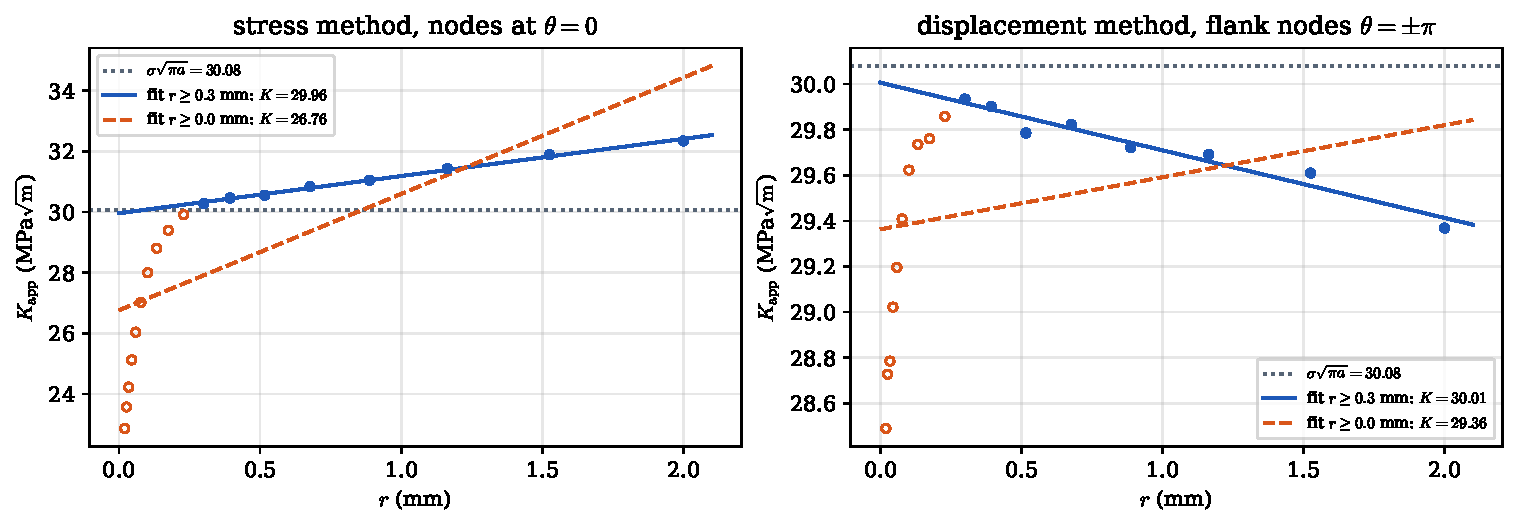
\includegraphics[width=\textwidth]{figures/extrapolation.pdf}
\caption{Extrapolation of the apparent $K$ to $r=0$. Open symbols are excluded from the solid fit;
including them (dashed) biases the result.}
\label{fig:extrap}
\end{figure}

\subsection{The $J$-integral alternative}
The $J$-integral is path-independent and is evaluated away from the tip, so it is less sensitive to the
mesh. For linear elastic mode I loading $J=G=K_I^2/E'$, hence $K_I=\sqrt{JE'}$.

%=====================================================================
\section{Using $K$: the fracture criterion}\label{sec:frac}
%=====================================================================
\subsection{Critical crack length}
Because $K$ fully describes the near-tip field, two cracks with the same $K$ are in the same state.
Fast fracture occurs when
\begin{equation}
  K_I = Y\sigma\sqrt{\pi a}\ \ge\ K_{IC},
  \qquad\Longrightarrow\qquad
  a_c = \frac1\pi\left(\frac{K_{IC}}{Y\sigma}\right)^2 .
\end{equation}
When $Y$ depends on $a/W$ this is solved numerically, for example by bisection on
$Y(a/W)\sigma\sqrt{\pi a}-K_{IC}=0$.

\subsection{The small-scale yielding principle}
The elastic solution predicts infinite stress at the tip, but a real metal yields. Linear elastic
fracture mechanics remains useful because of the \emph{small-scale yielding} (SSY) principle:

\begin{quote}
If the plastic zone at the tip is small compared with the crack length, the remaining ligament and
the thickness, it is embedded in a region where the elastic $K$ field still holds. That surrounding
$K$-dominated annulus then sets the boundary conditions on the plastic zone, so the state inside the
plastic zone, and hence whether the crack grows, is controlled by $K$ alone.
\end{quote}

Two cracks in different components with the same $K$ have identical plastic zones and fail at the same
$K$, even though neither is perfectly elastic. This \emph{autonomy} of the crack-tip region is what
allows a toughness $K_{IC}$ measured on a laboratory specimen to be used for a structure.

\begin{figure}[!htbp]
\centering
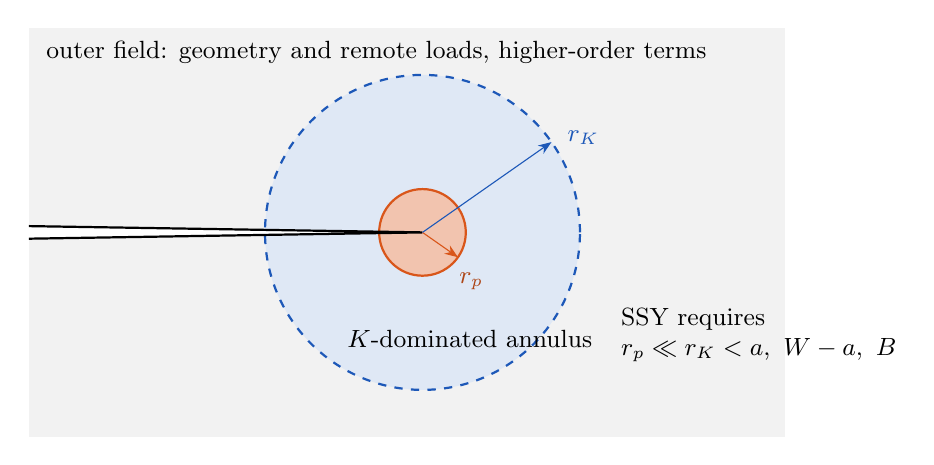
\begin{tikzpicture}[scale=1.0,>=Stealth]
  \fill[black!5] (-5,-2.6) rectangle (4.6,2.6);
  \node[font=\small,anchor=north west] at (-4.9,2.55) {outer field: geometry and remote loads, higher-order terms};
  \fill[accent!14] (0,0) circle (2.0);
  \fill[hot!35] (0,0) circle (0.55);
  \draw[accent,thick,dashed] (0,0) circle (2.0);
  \draw[hot,thick] (0,0) circle (0.55);
  \fill[white] (-5,0.08) -- (0,0) -- (-5,-0.08) -- cycle;
  \draw[thick] (-5,0.08) -- (0,0) -- (-5,-0.08);
  \node[font=\small,align=center] at (0.6,-1.35) {$K$-dominated annulus};
  \node[font=\small,hot!80!black] at (0.62,-0.62) {$r_p$};
  \draw[->,hot] (0,0) -- (-35:0.55);
  \draw[->,accent] (0,0) -- (35:2.0) node[pos=1.05,right,font=\small] {$r_K$};
  \node[font=\small,align=left,anchor=west] at (2.4,-1.3) {SSY requires\\$r_p \ll r_K < a,\ W-a,\ B$};
\end{tikzpicture}
\caption{Small-scale yielding: the plastic zone (radius $\sim r_p$) sits well inside the annulus where
$\sigma_{ij}\approx K f_{ij}(\theta)/\sqrt{2\pi r}$ is accurate. Outside $r_K$ the higher-order terms
of the Williams series matter.}
\label{fig:ssy}
\end{figure}

\subsection{Estimating the plastic zone}
\paragraph{First estimate.} Setting the elastic opening stress on $\theta=0$ equal to the yield
strength,
\begin{equation}
  \frac{K_I}{\sqrt{2\pi r_y}} = \sigma_{ys}
  \qquad\Longrightarrow\qquad
  r_y = \frac{1}{2\pi}\left(\frac{K_I}{\sigma_{ys}}\right)^2 .
\end{equation}
\paragraph{Irwin's correction.} The elastic stress above $\sigma_{ys}$ for $r<r_y$ (the shaded area in
Figure~\ref{fig:irwin}) cannot be carried by the yielded material, so it is redistributed further out.
Force balance makes the material behave as if the crack were longer, with an effective tip at
$a_{\rm eff}=a+r_y$, and doubles the zone:
\begin{equation}
  r_p = 2r_y = \frac{1}{\pi}\left(\frac{K_I}{\sigma_{ys}}\right)^2 \quad\text{(plane stress)},
  \qquad
  K_{\rm eff} = Y(a_{\rm eff})\,\sigma\sqrt{\pi a_{\rm eff}} .
\end{equation}
\paragraph{Plane strain.} Triaxial constraint raises the stress needed to yield, roughly to
$\sqrt3\,\sigma_{ys}$ ahead of the tip, giving
\begin{equation}
  r_p \approx \frac{1}{3\pi}\left(\frac{K_I}{\sigma_{ys}}\right)^2 \quad\text{(plane strain)}.
\end{equation}
\paragraph{Strip-yield (Dugdale) model.} Treating the plastic zone as a thin strip closed by a
cohesive stress $\sigma_{ys}$ gives, for small $\sigma/\sigma_{ys}$,
\begin{equation}
  \rho_D = \frac{\pi}{8}\left(\frac{K_I}{\sigma_{ys}}\right)^2 ,
\end{equation}
close to Irwin's $r_p$ ($\pi/8 = 0.39$ against $1/\pi = 0.32$).

\begin{figure}[!htbp]
\centering
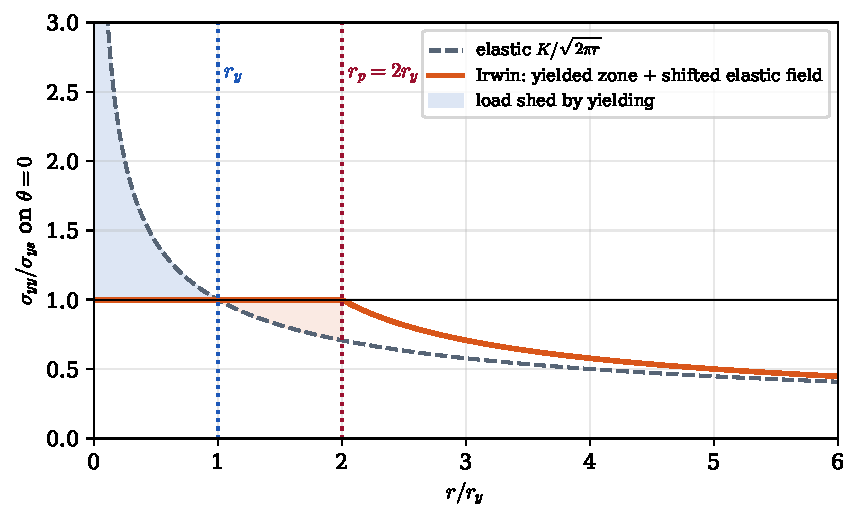
\includegraphics[width=.72\textwidth]{figures/irwin_profile.pdf}
\caption{Opening stress ahead of the tip with Irwin's correction. Yielding caps the stress at
$\sigma_{ys}$; the load shed for $r<r_y$ is carried between $r_y$ and $r_p=2r_y$, and beyond $r_p$
the elastic field is that of a crack with its tip moved forward by $r_y$.}
\label{fig:irwin}
\end{figure}

\subsection{When small-scale yielding holds}
\begin{itemize}
  \item The plastic zone must be small compared with every in-plane length: $r_p \ll a$ and
  $r_p \ll W-a$. A common rule of thumb is $r_p \lesssim a/50$ for an accurate $K$, and a plastic
  zone above about $0.1\,a$ makes LEFM doubtful. The pages flag this second limit.
  \item The applied stress must stay well below yield, typically $\sigma \lesssim 0.8\,\sigma_{ys}$ on
  the net section, otherwise the whole ligament yields.
  \item For a valid plane-strain $K_{IC}$ (ASTM E399) every dimension must be about 25 times the
  plane-strain plastic zone:
  \begin{equation}
    a,\ B,\ (W-a)\ \ge\ 2.5\left(\frac{K_{IC}}{\sigma_{ys}}\right)^2 .
  \end{equation}
\end{itemize}
When these conditions fail the regime is \emph{large-scale yielding}: $K$ no longer controls the
crack tip, and elastic--plastic parameters such as the $J$-integral or the crack-tip opening
displacement (CTOD) must be used instead. In the small-scale yielding limit they are related to
$K$ by $J = K_I^2/E'$ and $\delta_t \approx K_I^2/(m\,\sigma_{ys}E')$ with $m\approx1$ (plane
stress) to $2$ (plane strain).

\begin{table}[!htbp]
\centering
\caption{Typical teaching values (use certified data for design) and critical half crack length for the
centre crack with $W=200$\,mm, $\sigma=150$\,MPa.}
\begin{tabular}{@{}lccc@{}}
\toprule
Material & $K_{IC}$ ($\MPam$) & $\sigma_{ys}$ (MPa) & $a_c$ (mm)\\
\midrule
Al 7075-T6 & 29 & 505 & 11.7\\
AISI 4340, tempered 260\,\textdegree C & 50 & 1500 & 31.2\\
Ti-6Al-4V, annealed & 66 & 880 & 46.1\\
PMMA & 1.0 & 70 & ($\sigma>\sigma_{ys}$: LEFM not applicable)\\
\bottomrule
\end{tabular}
\end{table}

\paragraph{Example (Ti-6Al-4V).} At $a=20$\,mm, $K_I=38.6\MPam$, so $K_{IC}/K_I=1.71$ and
$r_p=(1/\pi)(38.6/880)^2=0.61$\,mm, which is 3\% of $a$: small-scale yielding holds. A valid
$K_{IC}$ test needs $B\ge2.5(66/880)^2=14.1$\,mm.

\begin{figure}[!htbp]
\centering
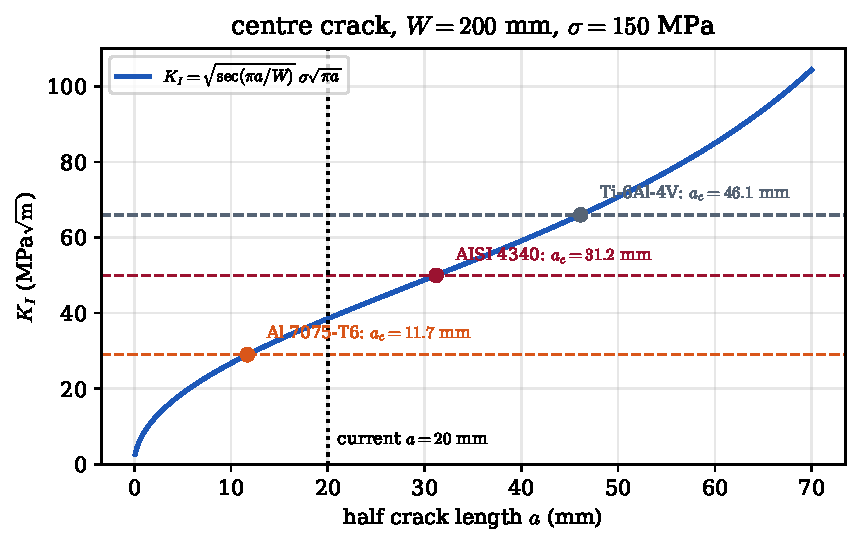
\includegraphics[width=.75\textwidth]{figures/fracture_curve.pdf}
\caption{$K_I$ against crack length compared with $K_{IC}$ for three materials.}
\end{figure}

%=====================================================================
\section{Angular functions for all modes}\label{sec:angular}
%=====================================================================
\subsection{What depends on geometry and what does not}
The angular functions $f_{ij}(\theta)$ are the same for every geometry; they change only with the
\emph{mode} of loading:
\begin{itemize}
  \item \textbf{Mode I} (opening): tension normal to the crack plane;
  \item \textbf{Mode II} (in-plane sliding): shear parallel to the crack, normal to the front;
  \item \textbf{Mode III} (tearing): out-of-plane shear, parallel to the front.
\end{itemize}
Geometry and load enter only through $K_I$, $K_{II}$, $K_{III}$ and through the higher-order terms,
starting with the $T$-stress. This remains true for an inclined crack, provided $\theta$ is measured in
the crack's own frame (Figure~\ref{fig:coords}). It does not hold for V-notches (the exponent and
angular functions depend on the notch angle), interface cracks between dissimilar materials, or
anisotropic materials.

\begin{table}[!htbp]
\centering
\caption{Mode I near-tip field.}\label{tab:modeI}
\renewcommand{\arraystretch}{1.5}
\begin{tabular}{@{}ll@{}}
\toprule
$\sigma_{xx}$ & $\dfrac{K_I}{\sqrt{2\pi r}}\cos\frac\theta2\left[1-\sin\frac\theta2\sin\frac{3\theta}2\right]$\\
$\sigma_{yy}$ & $\dfrac{K_I}{\sqrt{2\pi r}}\cos\frac\theta2\left[1+\sin\frac\theta2\sin\frac{3\theta}2\right]$\\
$\tau_{xy}$ & $\dfrac{K_I}{\sqrt{2\pi r}}\cos\frac\theta2\sin\frac\theta2\cos\frac{3\theta}2$\\
$\sigma_{rr}$ & $\dfrac{K_I}{\sqrt{2\pi r}}\left[\frac54\cos\frac\theta2-\frac14\cos\frac{3\theta}2\right]$\\
$\sigma_{\theta\theta}$ & $\dfrac{K_I}{\sqrt{2\pi r}}\left[\frac34\cos\frac\theta2+\frac14\cos\frac{3\theta}2\right]$\\
$\tau_{r\theta}$ & $\dfrac{K_I}{\sqrt{2\pi r}}\left[\frac14\sin\frac\theta2+\frac14\sin\frac{3\theta}2\right]$\\
$\sigma_{zz}$ & $0$ (plane stress), $\ \nu(\sigma_{xx}+\sigma_{yy})$ (plane strain)\\
$u_x$ & $\dfrac{K_I}{2\mu}\sqrt{\dfrac r{2\pi}}\cos\frac\theta2\left[\kappa-1+2\sin^2\frac\theta2\right]$\\
$u_y$ & $\dfrac{K_I}{2\mu}\sqrt{\dfrac r{2\pi}}\sin\frac\theta2\left[\kappa+1-2\cos^2\frac\theta2\right]$\\
\bottomrule
\end{tabular}
\end{table}

\begin{table}[!htbp]
\centering
\caption{Mode II near-tip field.}
\renewcommand{\arraystretch}{1.5}
\begin{tabular}{@{}ll@{}}
\toprule
$\sigma_{xx}$ & $-\dfrac{K_{II}}{\sqrt{2\pi r}}\sin\frac\theta2\left[2+\cos\frac\theta2\cos\frac{3\theta}2\right]$\\
$\sigma_{yy}$ & $\dfrac{K_{II}}{\sqrt{2\pi r}}\sin\frac\theta2\cos\frac\theta2\cos\frac{3\theta}2$\\
$\tau_{xy}$ & $\dfrac{K_{II}}{\sqrt{2\pi r}}\cos\frac\theta2\left[1-\sin\frac\theta2\sin\frac{3\theta}2\right]$\\
$\sigma_{rr}$ & $\dfrac{K_{II}}{\sqrt{2\pi r}}\left[-\frac54\sin\frac\theta2+\frac34\sin\frac{3\theta}2\right]$\\
$\sigma_{\theta\theta}$ & $\dfrac{K_{II}}{\sqrt{2\pi r}}\left[-\frac34\sin\frac\theta2-\frac34\sin\frac{3\theta}2\right]$\\
$\tau_{r\theta}$ & $\dfrac{K_{II}}{\sqrt{2\pi r}}\left[\frac14\cos\frac\theta2+\frac34\cos\frac{3\theta}2\right]$\\
$\sigma_{zz}$ & $0$ (plane stress), $\ \nu(\sigma_{xx}+\sigma_{yy})$ (plane strain)\\
$u_x$ & $\dfrac{K_{II}}{2\mu}\sqrt{\dfrac r{2\pi}}\sin\frac\theta2\left[\kappa+1+2\cos^2\frac\theta2\right]$\\
$u_y$ & $-\dfrac{K_{II}}{2\mu}\sqrt{\dfrac r{2\pi}}\cos\frac\theta2\left[\kappa-1-2\sin^2\frac\theta2\right]$\\
\bottomrule
\end{tabular}
\end{table}

\begin{table}[!htbp]
\centering
\caption{Mode III near-tip field (all in-plane stresses vanish).}
\renewcommand{\arraystretch}{1.5}
\begin{tabular}{@{}ll@{}}
\toprule
$\tau_{xz}$ & $-\dfrac{K_{III}}{\sqrt{2\pi r}}\sin\frac\theta2$\\
$\tau_{yz}$ & $\dfrac{K_{III}}{\sqrt{2\pi r}}\cos\frac\theta2$\\
$\tau_{rz}$ & $\dfrac{K_{III}}{\sqrt{2\pi r}}\sin\frac\theta2$\\
$\tau_{\theta z}$ & $\dfrac{K_{III}}{\sqrt{2\pi r}}\cos\frac\theta2$\\
$u_z$ & $\dfrac{2K_{III}}{\mu}\sqrt{\dfrac r{2\pi}}\sin\frac\theta2$\\
\bottomrule
\end{tabular}
\end{table}

The polar components follow from the Cartesian ones by rotation,
$\sigma_{rr}=\sigma_{xx}\cos^2\theta+\sigma_{yy}\sin^2\theta+2\tau_{xy}\sin\theta\cos\theta$,
$\sigma_{\theta\theta}=\sigma_{xx}\sin^2\theta+\sigma_{yy}\cos^2\theta-2\tau_{xy}\sin\theta\cos\theta$,
$\tau_{r\theta}=(\sigma_{yy}-\sigma_{xx})\sin\theta\cos\theta+\tau_{xy}(\cos^2\theta-\sin^2\theta)$;
the tables above were checked against this rotation numerically.

\begin{figure}[!htbp]
\centering
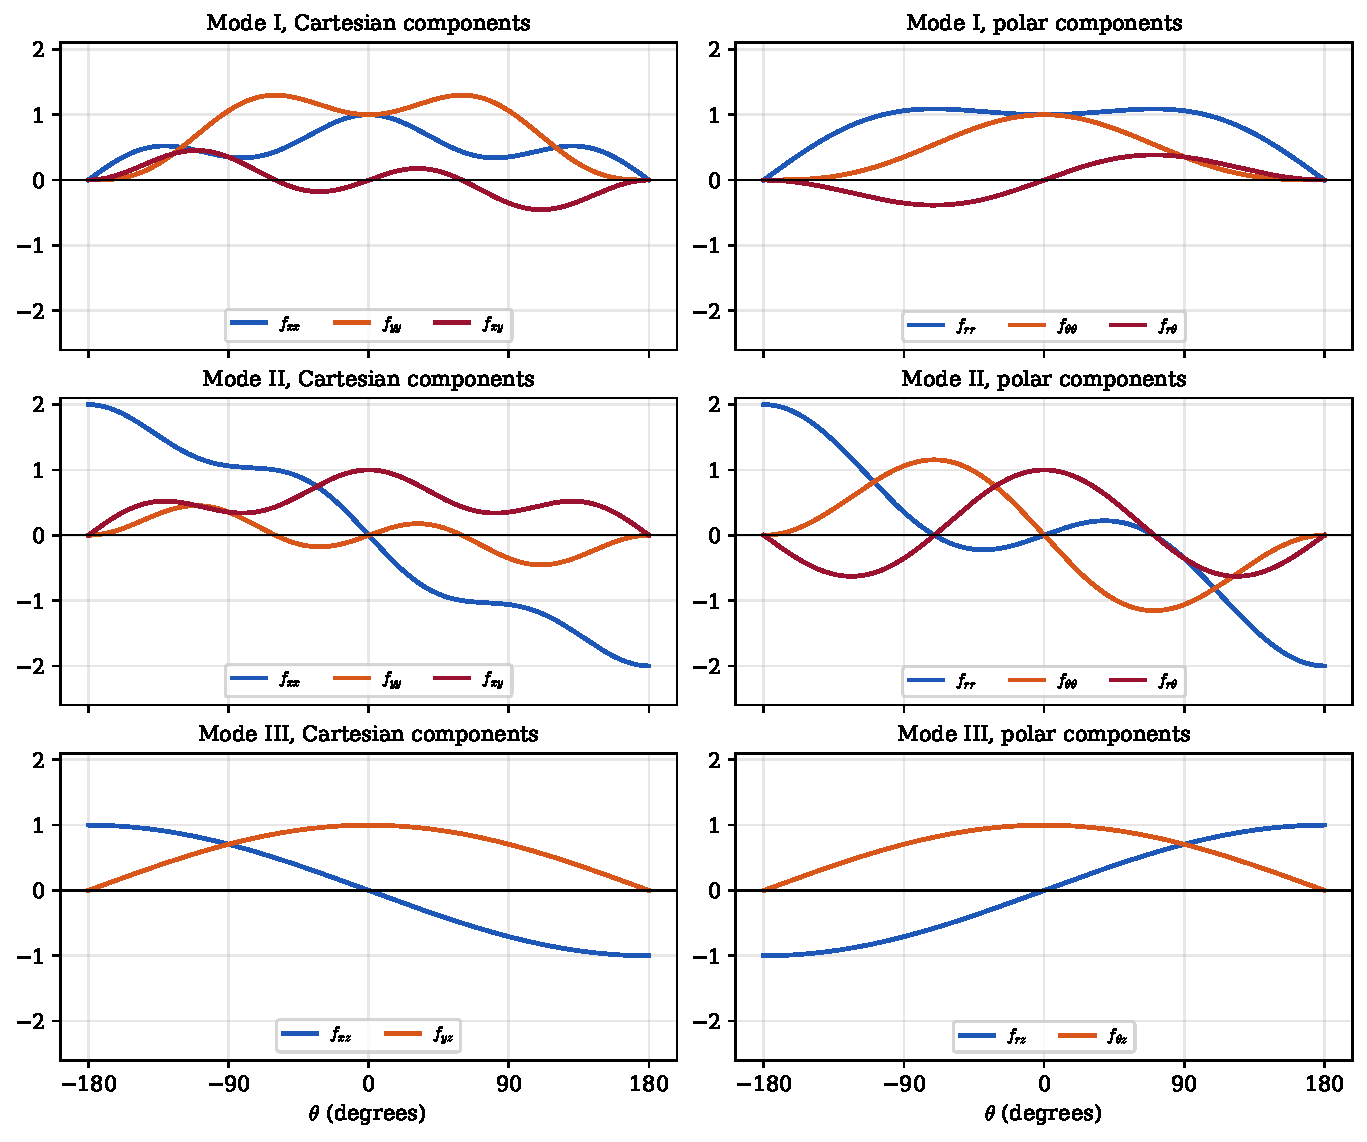
\includegraphics[width=\textwidth]{figures/angular_functions.pdf}
\caption{Angular functions $f_{ij}(\theta)$ for the three modes, from the lower crack face
($\theta=-180^\circ$) to the upper crack face ($\theta=+180^\circ$).}
\end{figure}

\subsection{Mixed-mode loading}
In linear elasticity the three fields superpose, each with its own $K$:
\begin{equation}
  \sigma_{ij} = \frac{1}{\sqrt{2\pi r}}\left[K_I f^{I}_{ij}(\theta)+K_{II} f^{II}_{ij}(\theta)+K_{III} f^{III}_{ij}(\theta)\right].
\end{equation}
The $K$'s themselves cannot be added because the angular functions differ, but the energy release rate
does add:
\begin{equation}
  G = \frac{K_I^2+K_{II}^2}{E'} + \frac{K_{III}^2}{2\mu}.
\end{equation}

\begin{table}[!htbp]
\centering
\caption{Loading cases and the modes they produce (through crack $2a$, infinite plate unless stated).}
\renewcommand{\arraystretch}{1.3}
\begin{tabular}{@{}llp{6.2cm}@{}}
\toprule
Geometry and loading & Mode & Stress intensity factors\\
\midrule
Tension normal to the crack plane & I & $K_I = Y\sigma\sqrt{\pi a}$\\
In-plane shear $\tau$ parallel to the crack & II & $K_{II}=\tau\sqrt{\pi a}$\\
Anti-plane shear $\tau$ (torsion of a cracked shaft) & III & $K_{III}=\tau\sqrt{\pi a}$\\
Crack at angle $\beta$ to uniaxial $\sigma$ & I + II & $K_I=\sigma\sqrt{\pi a}\sin^2\beta$, $K_{II}=\sigma\sqrt{\pi a}\sin\beta\cos\beta$\\
Tension plus torsion on a cracked tube & I + III & superpose the two solutions\\
\bottomrule
\end{tabular}
\end{table}

For the inclined crack, $\beta$ is the angle between the crack line and the load:
$\beta=90^\circ$ gives pure mode I and $\beta=45^\circ$ gives $K_I=K_{II}=\tfrac12\sigma\sqrt{\pi a}$.

\subsection{The $T$-stress}
The full Williams expansion for mode I is
\begin{equation}
  \sigma_{ij} = \frac{K_I}{\sqrt{2\pi r}}f^{I}_{ij}(\theta) + T\,\delta_{1i}\delta_{1j} + O(\sqrt r).
\end{equation}
$T$ is a constant stress parallel to the crack (it adds only to $\sigma_{xx}$). It depends on geometry
and loading, and it controls crack-tip constraint and the size of the zone in which $K$ alone describes
the field.

\begin{table}[!htbp]
\centering
\caption{$T$-stress for a through crack $2a$ in an infinite plate.}
\begin{tabular}{@{}lc@{}}
\toprule
Loading & $T$\\
\midrule
Uniaxial $\sigma$ normal to the crack & $-\sigma$\\
Equibiaxial $\sigma$ & $0$\\
Uniaxial $\sigma$ at angle $\beta$ to the crack line & $\sigma\cos2\beta$\\
\bottomrule
\end{tabular}
\end{table}
For finite specimens $T$ is usually given through the biaxiality ratio $B=T\sqrt{\pi a}/K_I$
(Leevers and Radon 1982; Sherry et al.\ 1995).

\paragraph{Physical meaning.} $T$ is a uniform stress acting parallel to the crack. It is the same at every
distance $r$ and is set by the remote loading and the geometry, not by the singularity. Deep edge cracks in
bending (SENB, CT) have $T>0$; short cracks and centre-cracked panels in tension have $T<0$.

\paragraph{Why $T$ does not change $J$ or $G$.} A stress parallel to the crack does not open the crack faces,
so it releases no energy at the tip. In the $J$-integral the $T^2$ part is a uniform field with no singularity
inside the contour and integrates to zero, and the $K_I T$ cross term cancels between the upper and lower
halves of the contour by symmetry. Hence $J=K_I^2/E'$ for any $T$; only the split between the
$\int W\,\mathrm dy$ and $-\int T_i\,\partial u_i/\partial x\,\mathrm ds$ terms changes.
(Here $T_i=\sigma_{ij}n_j$ is the traction vector, a different quantity from the scalar $T$-stress.)

\paragraph{Constraint.} $T$ changes the stress triaxiality ahead of the tip (Larsson and Carlsson 1973).
\begin{itemize}
  \item $T>0$, high constraint: higher hydrostatic stress, a smaller plastic zone that leans forward, and
  toughness close to the lower bound. Deep-cracked test specimens are in this regime.
  \item $T<0$, loss of constraint: lower hydrostatic stress, a larger plastic zone, and an apparent toughness
  above $K_{IC}$ or $J_{Ic}$. Shallow cracks and thin panels in tension are in this regime.
\end{itemize}
Two cracks with the same $K$ or $J$ can therefore fail at different loads. This is the basis of two-parameter
fracture mechanics: $K$--$T$ or $J$--$T$ (Beteg\'on and Hancock 1991) and $J$--$Q$ (O'Dowd and Shih 1991).

\paragraph{Crack path.} $T$ also controls directional stability: with $T>0$ a straight crack tends to kink
out of its plane, with $T<0$ it stays straight (Cotterell and Rice 1980).

%=====================================================================
\section*{References}
\addcontentsline{toc}{section}{References}
\begin{itemize}
  \item C.~E. Inglis (1913). Stresses in a plate due to the presence of cracks and sharp corners.
  \emph{Trans.\ Inst.\ Naval Architects} 55, 219--241.
  \item N.~I. Muskhelishvili (1953). \emph{Some Basic Problems of the Mathematical Theory of Elasticity}. Noordhoff.
  \item H.~M. Westergaard (1939). Bearing pressures and cracks. \emph{J.\ Appl.\ Mech.} 6, A49--A53.
  \item M.~L. Williams (1957). On the stress distribution at the base of a stationary crack.
  \emph{J.\ Appl.\ Mech.} 24, 109--114.
  \item G.~R. Irwin (1957). Analysis of stresses and strains near the end of a crack traversing a plate.
  \emph{J.\ Appl.\ Mech.} 24, 361--364.
  \item H.~Tada, P.~C. Paris, G.~R. Irwin (2000). \emph{The Stress Analysis of Cracks Handbook}, 3rd ed. ASME.
  \item T.~L. Anderson (2017). \emph{Fracture Mechanics: Fundamentals and Applications}, 4th ed. CRC Press.
  \item ASTM E399. Standard test method for linear-elastic plane-strain fracture toughness of metallic materials.
  \item C.~E. Feddersen (1967). Discussion of plane strain crack toughness testing. \emph{ASTM STP 410}, 77--79.
  \item D.~S. Dugdale (1960). Yielding of steel sheets containing slits. \emph{J.\ Mech.\ Phys.\ Solids} 8, 100--104.
  \item P.~S. Leevers, J.~C. Radon (1982). Inherent stress biaxiality in various fracture specimen geometries. \emph{Int.\ J.\ Fract.} 19, 311--325.
  \item A.~H. Sherry, C.~C. France, M.~R. Goldthorpe (1995). Compendium of T-stress solutions for two and three dimensional cracked geometries. \emph{Fatigue Fract.\ Eng.\ Mater.\ Struct.} 18, 141--155.
  \item J.~R. Rice (1968). A path independent integral and the approximate analysis of strain concentration by notches and cracks. \emph{J.\ Appl.\ Mech.} 35, 379--386.
  \item S.~G. Larsson, A.~J. Carlsson (1973). Influence of non-singular stress terms and specimen geometry on small-scale yielding at crack tips in elastic--plastic materials. \emph{J.\ Mech.\ Phys.\ Solids} 21, 263--277.
  \item C.~Beteg\'on, J.~W. Hancock (1991). Two-parameter characterization of elastic--plastic crack-tip fields. \emph{J.\ Appl.\ Mech.} 58, 104--110.
  \item N.~P. O'Dowd, C.~F. Shih (1991). Family of crack-tip fields characterized by a triaxiality parameter---I. Structure of fields. \emph{J.\ Mech.\ Phys.\ Solids} 39, 989--1015.
  \item B.~Cotterell, J.~R. Rice (1980). Slightly curved or kinked cracks. \emph{Int.\ J.\ Fract.} 16, 155--169.
  \item A.~A. Griffith (1921). The phenomena of rupture and flow in solids. \emph{Phil.\ Trans.\ R.\ Soc.\ A} 221, 163--198.
\end{itemize}

\end{document}
